\chapter{Fonctionnalités}
\label{s:fonctionnalite}

\section{Image}
\subsection{Importation}
Non implémenté

\subsection{Exportation}
Implémenté

\subsection{Espace de couleur}
Implémenté

\subsection{Traitement d'image}
Une catégorie situé au coin droit de l’écran permet l’utilisation de plusieurs filtres s’affichant sur l’entièreté de la scène. Elle regroupe trois type de filtres: le brouillage (Blur), l’inversement des couleurs et la dilatation. Les trois filtres peuvent être appliqués tous en même temps ou un à la fois.\\

Un objet ofxCvColorImage est utilisé pour la réalisation des filtres. On capture les pixels de la scène et on l’ajoute dans cet objet, pour ensuite lui faire subir les filtres sélectionnés par l’utilisateur. Les fonctions blur(), invert() et dilate() on été utilisées pour construire le filtre. Ces fonctions utilisent différentes opérations sur chaque pixel de l’image pour les modifier.\\

Voici une image d’une scène avec des filtres d’inversement de couleurs et de brouillage:\\
\begin{figure}[h]
	\centering
	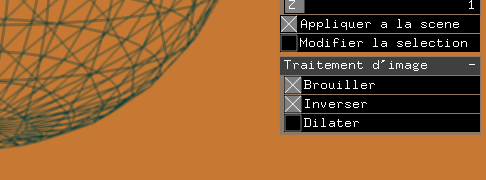
\includegraphics[width=5cm]{fig/filters.png}
	\caption{Une scène avec filtres.}
	\label{fig:filtres}
\end{figure}


\subsection{Image procédurale}
Non implémenté

\pagebreak
\section{Dessin vectoriel}
\subsection{Curseur dynamique}
Implémenté

\subsection{Primitives vectorielles}
Implémenté

\subsection{Formes vectorielles}

\begin{figure}[h]
	\centering
	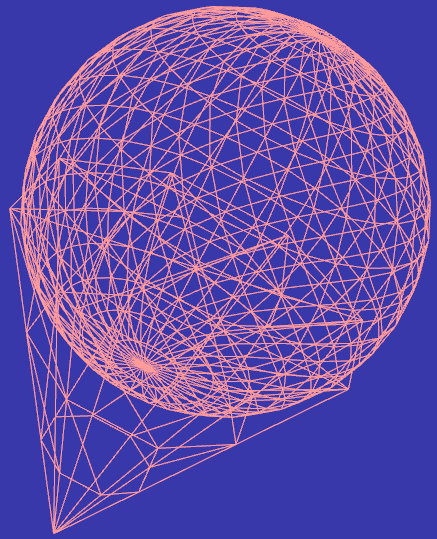
\includegraphics[width=5cm]{fig/iceCream.png}
	\caption{Cornet de crème glacé!}
	\label{fig:iceCream}
\end{figure}

\subsection{Outils de dessin}
Implémenté

\subsection{Interface}
Implémenté

\pagebreak
\section{Transformation}
\subsection{Transformation interactive}
Une catégorie à droite de l’application permet de transformer le systèmes de coordonnées des entités géométriques de la scène. On peut exercer des transformations tel que la translation en X, Y et Z, la rotation en X, Y et Z ainsi que la proportion en X, Y et Z. Elle peut se faire autant en temps réel qu’en différé. \\

Les matrices de transformation d’openframeworks sont utilisés pour la réalisation des transformations. On utilise les méthodes ofPushMatrix() et ofPopMatrix(). Une fois la matrice empilé, on ajoute les transformation à l’aide des méthodes ofTranslate(), ofRotate() et ofScale() selon les paramètres inscrit par l’utilisateur. Enfin, on dépile la matrice pour permettre la transformation.\\

Voici le menu des transformations et ces différentes options:\\
\begin{figure}[h]
	\centering
	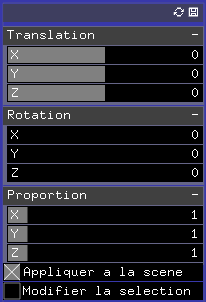
\includegraphics[width=5cm]{fig/transformations.png}
	\caption{Menu des transformations.}
	\label{fig:transformations}
\end{figure}

\subsection{Structure de scène}
La structure de scène a été implémenté sous la forme d'un arbre ordoné, dans lequel les feuilles sont les éléments de la scène. La classe scène comprend 4 classes interne, soit element, group, node et scene\_iterator. Les classes group et node héritent d'element et  servent à stocker tout ce qui se trouve dans la scène. La classe scene\_iterator permet, quant-à elle, de parcourir les éléments pour les dessiner. 

On utilise les shared\_ptr au lieux des simples pointeurs pour conserver les éléments qui sont ajouté à la scène pour ne pas avoir à trop gérer la mémoire.

L'essentiel du code de la scène se trouve dans les méthodes addElement de la scène, des sous-clases de stockage et l'operator++ de l'itérateur.

\begin{lstlisting}
void scene::addElement(size_t index, primitive_ptr& p, bool insertFirstChild) {
	if (index == 0 && !insertFirstChild {
		throw invalid_argument("root don't have parent...");
	}
	root->addElement(index, p, insertFirstChild);
}

//Retourne la quantite d'element ajoute
size_t scene::node::addElement(size_t index, primitive_ptr& p, bool insertFirstChild) {
	if (index != this->index) {
		throw invalid_argument("index need to be equals to the index of the node");
	}
	if (insertFirstChild) {
		throw invalid_argument("node need to be wraped in a group");
	}
	this->content = p;
	contentType = "primitive";
	return 1;
}

//Retourne la quantite d'element ajoute
size_t scene::group::addElement(size_t index, primitive_ptr& p, bool insertFirstChild) {
	size_t addedSize = 0;
	
	if (this->index == index) {
		if (insertFirstChild) {
			//Inserer comme premier element
			childrens.insert(childrens.begin(), element_ptr{ new node{ index + 1, height + 1, p } });
			for (auto& it = childrens.begin() + 1; it < childrens.end(); ++it) {
				it->get()->setIndex(it->get()->getIndex() + 1);
			}
			addedSize++;
		} else {
			throw invalid_argument("element must to be add in the parent");
		}
	} else {
		size_t ubound = childrens.size();
		size_t lbound = 0;
		size_t i;
		
		//Recherche binaire
		while (lbound <= ubound) {
			i = lbound + (ubound - lbound) / 2;
			if (childrens[i]->getIndex() == index) {
				if (insertFirstChild) {
					if (childrens[i]->getType() != "group") {
						group_ptr temp = group_ptr{ new group{ index, height + 1 } };
						temp->childrens.push_back(childrens[i]);
						temp->childrens[0]->setIndex(index + 1);
						temp->childrens[0]->setHeight(height + 2);
						temp->size = temp->childrens[0]->getSize() + 1;
						childrens[i] = temp;
						addedSize++;
					}
					addedSize += childrens[i]->addElement(index, p, insertFirstChild);
				} else {
					childrens.insert(childrens.begin() + i + 1, element_ptr{ new node{ index + childrens[i]->getSize(), height + 1, p } });
					i++;
					addedSize++;
				}
				i++;
				break;
			} else if (childrens[i]->getIndex() < index) {
				lbound = i + 1;
				if (ubound < lbound) {
					//Ajoute l'element dans le groupe sous-jacent
					addedSize += childrens[i]->addElement(index, p, insertFirstChild);
					i++;
					break;
				}
			} else {
				ubound = i - 1;
				if (ubound < lbound) {
					//Ajoute l'element dans le groupe sous-jacent
					addedSize += childrens[i - 1]->addElement(index, p, insertFirstChild);
					break;
				}
			}
		}	
		for (auto& it = childrens.begin() + i; it < childrens.end(); ++it) {
			it->get()->setIndex(it->get()->getIndex() + addedSize);
		}
	}
	size += addedSize;
	return addedSize;
}

//Avance jusqu'au prochain node
void scene::scene_iterator::operator++() {
	for (rootIndex; rootIndex <= root->getSize(); ++rootIndex) {
		element* elem = root->getElement(rootIndex);
		if (elem->getType() != "group" && elem->getType() != "root") {
			primitive_ptr ptr = (dynamic_cast<node*>(elem))->content;
			if (p != ptr) {
				p = ptr;
				break;
			}
		}
	}
	if (rootIndex > root->getSize()) {
		p = primitive_ptr{ nullptr };
	}
}
\end{lstlisting}
Comme vous avez sans-doute remarqué, l'ajout d'élément à la scène se fait récursivement, à l'index en paramètre. Le paramètre «insertFirstChild» indique s'il faut insérer l'élément comme le premier enfant de l'élément à l'index en paramètre. S'il est faux, on insère simplement le nouvel élément après l'index. Dans group::addElement, on utilise un algorithme de recherche binaire pour trouver dans ou après quel élément il faut ajouter le nouvel élément.

L'operator++, quant à lui, parcours la scène en s'arrêtant seulement sur les classes node.  

Malheureusement, par manque de temps la structure de scène n'est pas utilisé à sont plein potentiel et tous les éléments sont stocké dans le groupe à la racine de la scène. Il est tout de même possible de voir le résultat en changeant la ligne «\#define test 0» pour «\#define test 1» dans le fichier «main.cpp». Vous verrez alors le résultat de l'exécution des tests de la classe scene (principalement de l'ajout et de la supression d'élément), se trouvant à la fin de «scene.cpp». 

\subsection{Sélection multiple}
Implémenté

\subsection{Coordonnées non-cartésiennes}
Non-implémenté

\subsection{Historique}
Non-implémenté

\pagebreak
\section{Géométrie}
\subsection{Particules}
Non-implémenté

\subsection{Primitives}

\large{Primitives 2D:}\\
Dans les types de primitives disponibles, on trouve la catégorie 2D. En sélectionnant cette catégorie, on peut ainsi dessiner des carrés, des cercles (ellipses), des triangles, des lignes et des points. Toutes ces primitives sont affectés par la position, la taille, l’épaisseur de traits, la couleur de remplissage et de bordure ainsi que la texture passé par l’utilisateur.\\

Des objets ofPath sont utilisés pour toute les types de primitives 2d créer. Afin d’avoir une meilleure intégration à la scène, une casse générique de primitives 2d a été créer. Pour les différents types, différentes méthodes ont été conçu pour créer les primitives. Ces méthodes utilisent les méthodes ellipse(), circle(), rect(), triangle() et line(). Elles appliquent chaque propriétés spécifiés par l’utilisateur. Après chaque ajout, on ajoute ensuite les primitives dans la scène.\\

Voici à quoi ressemble les différentes primitives 2D:\\
\begin{figure}[h]
	\centering
	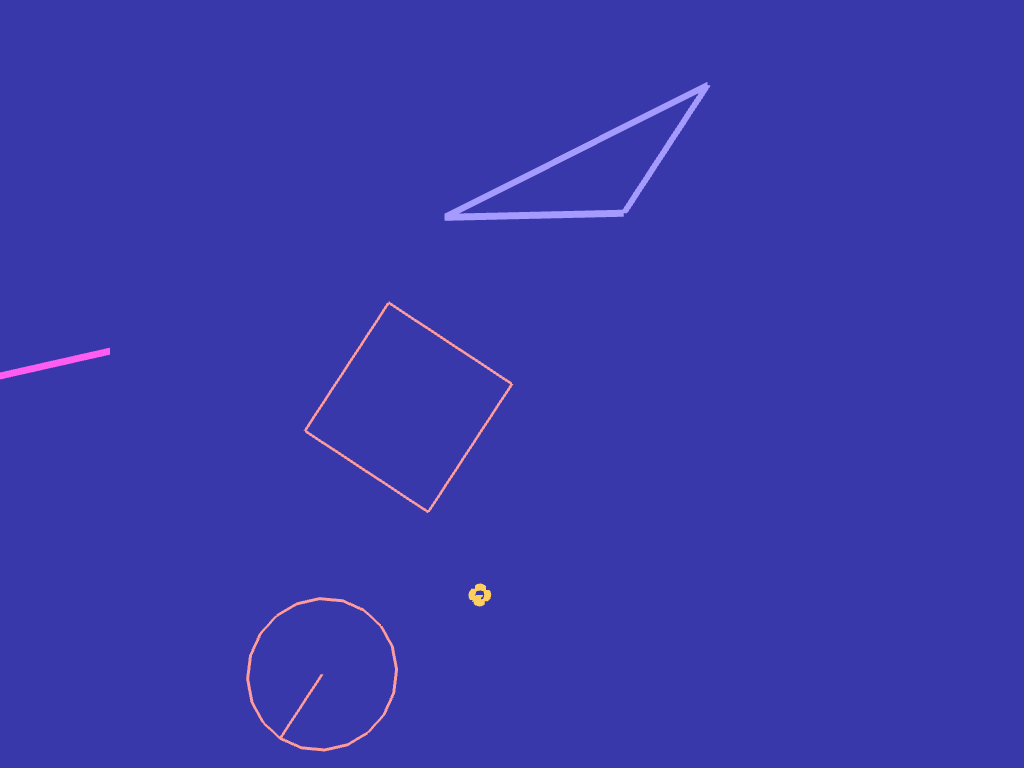
\includegraphics[width=5cm]{fig/primitives2d.png}
	\caption{Une scène avec primitives 2d.}
	\label{fig:prim2d}
\end{figure}

\subsection{Modèle}
Implémenté

\subsection{Texture}
Implémenté

\subsection{Géométrie procédurale}
Non-implémenté

\pagebreak
\section{Caméra}
\subsection{Propriétés de caméra}
Les propriétés de la caméra tel que le champ de vision, le ratio d'aspect ainsi que la distance du plan de clipping avant et arrière. Ils peuvent être modifier dans l'interface graphique à l'aide de slider. L'essentiel du code se trouve dans «ccamera::update()».


\begin{lstlisting}
	cam->setFov(fov.get());
	if (autoRatio.get()) {
		cam->setForceAspectRatio(false);
	} else {
		cam->setAspectRatio(ratio.get());
	}
	cam->setNearClip(nearClip.get());
	cam->setFarClip(farClip.get());
\end{lstlisting}

\begin{figure}[h]
	\centering
	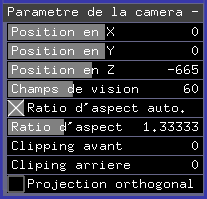
\includegraphics[width=5cm]{fig/proprieteCamera.png}
	\caption{Propriété de la caméra dans l'interface}
	\label{fig:propriete}
\end{figure}

\subsection{Mode de projection}
Le changement de mode de projection de perspective à orthogonale a été implémenté dans l'application. L'essentiel du travail se fait dans la méthode «ccamera::changeMode()». Elle est appelé lorsqu'on appuit sur le bouton à cet effet dans l'interface graphique.

\begin{lstlisting}
	if (ortho.get()) {
		cam->enableOrtho();
	} else {
		cam->disableOrtho();
	}
\end{lstlisting}

\subsection{Caméra interactive}
La caméra interactive est implémenter dans l'application principalement à l'aide de la classe ofEasyCam de openFrameworks. Nous avons tout de même ajouter la possibilité de déplacer à l'aide des flèches du clavier, pour permettre de repositionner facilement la caméra. Il est aussi possible d'avancer à caméra à l'aide de pageUp/Down. L'essentiel du code se trouve au début de «ccamera::update()».

\begin{lstlisting}
	float dist = speed * dt;
	float dx = 0;
	float dy = 0;
	float dz = 0;
	
	dx = 0;
	if (isCameraMoveLeft)
		dx += dist;
	if (isCameraMoveRight)
		dx -= dist;
	cam->truck(-dx);
	posX.set(round(-cam->getX()));
	
	dy = 0;
	if (isCameraMoveUp)
		dy -= dist;
	if (isCameraMoveDown)
		dy += dist;
	cam->boom(-dy);
	posY.set(round(cam->getY()));
	
	dz = 0;
	if (isCameraMoveForward)
		dz -= dist;
	if (isCameraMoveBackward)
		dz += dist;
	cam->dolly(dz);
	posZ.set(round(cam->getZ()));
\end{lstlisting}

\subsection{Caméra multiple}
Non-implémenté

\subsection{Caméra animée}
Non-implémenté
